\documentclass{article} % For LaTeX2e
\usepackage[submission]{colm2026_conference}

\usepackage{microtype}
\usepackage{hyperref}
\usepackage{url}
\usepackage{booktabs}
\usepackage{lineno}
\usepackage{amsmath}
\usepackage{amssymb}
\usepackage{amsfonts}
\usepackage{graphicx}
\usepackage{longtable}
\usepackage{array}
\usepackage{pdflscape}

\input{math_commands.tex}

\definecolor{darkblue}{rgb}{0, 0, 0.5}
\hypersetup{colorlinks=true, citecolor=darkblue, linkcolor=darkblue, urlcolor=darkblue}

\title{ATMA: Length-Invariant Language Modeling via Polar Attention and Gated-Delta Compression Memory}

% Authors must not appear in the submitted version for COLM.
\author{Anonymous Authors \\
Paper Under Review for COLM Workshop
}

\newcommand{\fix}{\marginpar{FIX}}
\newcommand{\new}{\marginpar{NEW}}

\begin{document}

\ifcolmsubmission
\linenumbers
\fi

\maketitle

\begin{abstract}
Modern large language models based on softmax scaled-dot-product attention are fundamentally constrained by their training sequence length. As the key-value sequence grows, the softmax probability mass dilutes across a wider distribution, causing a breakdown of in-distribution activations and severe performance collapse under sequence length extrapolation. Moreover, long-context language modeling faces a structural tension: a sliding-window attention core maintains a bounded local representation and low perplexity but is blind to long-range dependencies, while full-context attention preserves global recall but suffers from out-of-distribution perplexity explosion. To resolve these limitations, we introduce \textbf{ATMA}, a hybrid convolutional-attention architecture that integrates a novel three-channel attention mechanism. ATMA factorizes the attention mixing step into: (1) a count-blind, unit-vector \textbf{direction} channel, (2) a bounded \textbf{magnitude} channel driven by the participation ratio of effective matches over an extreme-value-corrected null sink, and (3) a long-term \textbf{recurrent compression memory} optimized via a gated-delta fast-weights rule. This multi-channel decomposition enables ATMA to achieve monotonic perplexity reduction and high-fidelity long-range retrieval simultaneously. We evaluate ATMA using a massive 100-run factorial ablation sweep, demonstrating that it maintains induction needle-in-a-haystack retrieval accuracy above 90\% out to 64K tokens (32$\times$ the training length of 2K) while its document perplexity improves monotonically, significantly outperforming softmax-based memory baselines which collapse at extreme context lengths.
\end{abstract}

\section{Introduction}

\begin{figure}[t!]
\centering

\includegraphics[width=0.88\linewidth]{fig_niah.pdf}
\caption{Induction Needle-in-a-Haystack (NIAH) retrieval accuracy comparison under context length extrapolation (up to 32$\times$ the training sequence length of 2,048 tokens). Only ATMA (Polar + Titans Memory) holds flat accuracy above 90\% out to 64K, whereas all other configurations collapse.}
\label{fig:niah}
\end{figure}

The capacity of Large Language Models (LLMs) to ingest, process, and reason over massive context windows is a cornerstone of modern artificial intelligence capabilities. Applications ranging from repository-level code synthesis to complex academic document analysis depend on the model's ability to maintain coherent representations across tens of thousands of tokens. However, the standard sequence mixer, Softmax Scalable-Dot-Product Attention (SDPA)~\citep{Vaswani+2017}, exhibits severe limitations when generalizing to sequence lengths beyond those encountered during training.

This failure of length extrapolation stems from two distinct mathematical properties of softmax attention. First, softmax attention is \textbf{not length-invariant}. As the number of keys $N$ grows, the probability mass is distributed across a larger population, causing the individual attention weights to dilute toward zero (the "dilution" problem). Consequently, a model trained at length $T$ experiences a dramatic shift in its activation distribution when evaluated at $32\cdot T$. Second, softmax attention entangles magnitude information (``how many items matched the query'') with direction information (``what features were matched'') into a single normalized output. When evaluated at longer contexts, the accumulated representations shift the residual stream's DC level, pushing downstream feed-forward networks out-of-distribution.

Faced with this challenge, practitioners often employ Sliding Window Attention (SWA)~\citep{beltagy2020longformer} or Recurrent/Linear Attention alternatives~\citep{deltanet2024, mamba2023}. However, this introduces a severe trade-off:
\begin{itemize}
    \item \textbf{Sliding Window Attention} keeps the active key set bounded and thus maintains excellent local perplexity, but it is completely blind to any retrieval targets located past the window boundary.
    \item \textbf{Full Softmax Attention} preserves distant recall under specialized conditions, but suffers from severe perplexity collapse as the cumulative attention activations explode and drift.
    \item \textbf{Recurrent Fast-Weight Memories} act as lossy compression systems that carry general document flow, but lack the high-precision focus required to recall random, pinpoint facts (the ``needle-in-a-haystack'' problem) from a massive context.
\end{itemize}

We resolve this tension by introducing \textbf{ATMA}, a hybrid sequence-modeling architecture that merges the structural local-mixing advantages of gated depthwise convolutions with a novel three-channel attention layer. In ATMA, each attention layer decomposes its output into an additive combination of three distinct streams:
\begin{equation}
    \mathbf{out} = \mathbf{content} + \mathbf{count} + \mathbf{memory}
\end{equation}
The first two streams (\textbf{content} and \textbf{count}) form our proposed \textbf{Polar Attention} core. By projecting the matched value-sum onto the unit sphere, the \textbf{content} channel isolates \textit{what} matched, resulting in a count-blind, size-invariant direction vector. Concurrently, the \textbf{count} channel isolates \textit{how much} matched by calculating the participation ratio (inverse Simpson index) of the attention distribution, bounded via a saturating monotonic map. To prevent background noise from overwhelming the signal at extreme sequence lengths, Polar Attention calibrates its logits against a learned, extreme-value-corrected null floor that tracks the expected maximum of random scores.

The third stream (\textbf{memory}) is a recurrent, per-head associative memory block driven by a gated-delta update rule, inspired by the Titans model~\citep{titans2025}. The linear memory behaves as a lossy gist that captures long-term perplexity trends, allowing the Polar Attention core to be paired with a sliding window for local modeling while the memory maintains global context. When exact global recall is required, full Polar Attention can be enabled; since its representations are length-invariant, it Generalizes to extreme lengths without activation drift.

To rigorously validate our architectural design, we perform a \textbf{100-run factorial ablation sweep}, training 370M-parameter models on a 1-billion token Fineweb-Edu corpus, and evaluating them across context lengths from 2K to 64K tokens (up to 32$\times$ training length). The results show a clear hierarchy: the combination of Polar Attention and Titans memory completely eliminates the window-vs-retrieval trade-off. ATMA models hold induction needle-in-a-haystack retrieval flat above 90\% across the entire 2K$\to$64K sweep while clean-document perplexity improves monotonically, outperforming both vanilla softmax and softmax-recurrent hybrid baselines.

Our implementation is optimized and numerically cross-verified across three parallel pipelines: a pure-PyTorch reference, an FP16/FP8 training harness, and a paged inference engine. We introduce a FlashAttention-style Triton kernel that handles the streaming participation-ratio calculations in $O(\text{block})$ memory, and we wrap the fast gated-delta training recurrence as opaque custom ops to avoid dynamo compiler graph breaks. This codesign reduces the computational overhead of the memory branch to a mere 6--9\% relative MFU.

\section{Related Work}

\subsection{Softmax Attention and Scaling Limits}
Traditional Transformer architectures rely on softmax scaled-dot-product self-attention~\citep{Vaswani+2017}. While highly expressive, the $O(T^2)$ computational complexity has inspired numerous long-context extensions. Positional representations like Rotary Position Embeddings (RoPE)~\citep{rope2021} and Attention with Linear Biases (ALiBi)~\citep{alibi2021} allow models to extrapolate position indicators to longer sequences. However, they do not resolve the fundamental issue of softmax dilution: as sequence length increases, the attention probability assigned to relevant keys is systematically diluted by the growing number of irrelevant distractors. This leads to severe retrieval degradation at long distances. Sliding Window Attention (SWA)~\citep{beltagy2020longformer} avoids this dilution by truncating the attention context, but permanently sacrifices long-range recall.

\subsection{Linear Attention and Recurrent Fast Weights}
To achieve linear-time complexity, linear attention reformulates attention by shifting the computation order of the key, query, and value matrices~\citep{deltanet2024}. This reparametrization effectively treats the sequence mixer as a recurrent neural network with a matrix-valued state. Recent models like Gated DeltaNet~\citep{deltanet2024} and Titans~\citep{titans2025} incorporate data-dependent gating and delta-rule updates to actively overwrite and retrieve memories. Titans, in particular, proposes a ``Memory-as-Gate'' (MAG) or ``Memory-as-Layer'' approach to store historical context. However, purely linear recurrent states are fundamentally limited by their storage capacity ($O(d_k \cdot d_v)$ parameters); they act as lossy compression systems that struggle to exact-recall rare pinpoint facts (needles) out of massive text haystacks.

\subsection{Hybrid Architectures and Canon Layers}
Recent work demonstrates that hybrid architectures combining local and global sequence mixers can outperform pure transformers on both efficiency and quality. Models like Mamba~\citep{mamba2023} and Liquid Foundation Models 2 (LFM2)~\citep{lfm2_2025} combine linear state-space models or gated convolutions with sparse attention layers. Furthermore, \citet{physics_lms_2025} show that incorporating depthwise causal convolutions (known as Canon layers) on the query, key, and value projections prior to scoring provides critical horizontal shift-covariance and spatial awareness. ATMA builds on these insights, adopting a 3:1 ratio of LFM2 convolutions to Polar Attention layers to maximize parameter efficiency and sequence throughput.

\section{Methodology}

\subsection{Architecture Overview}
ATMA is a 16-layer decoder-only language model designed with a 3:1 hybrid sequence-mixing ratio. Specifically, the architecture consists of 12 LFM2 gated convolutional layers and 4 Polar Attention layers. Each decoder block uses a pre-normalization layout:
\begin{align}
    x' &= x + \operatorname{SubLayer}(\operatorname{RMSNorm}(x)) \\
    x'' &= x' + \operatorname{MLP}(\operatorname{RMSNorm}(x'))
\end{align}
where the SubLayer is either an LFM2 gated convolution or a Polar Attention layer. The MLP block uses a squared-ReLU activation function with a 4$\times$ hidden dimension expansion:
\begin{equation}
    \operatorname{MLP}(z) = W_{\text{down}}\left( \operatorname{ReLU}(W_{\text{gate}} z)^2 \cdot (W_{\text{up}} z) \right)
\end{equation}
By keeping the attention footprint sparse (only 4 out of 16 layers), ATMA maintains low computational overhead while leveraging the global mixing capacity of Polar Attention and Titans memory.

\subsection{Polar Attention}
Polar Attention is a length-invariant replacement for softmax scaled-dot-product attention. It operates within the standard Grouped-Query Attention (GQA) framework, with $H$ query heads and $H_{\text{KV}} = H / 4$ key-value heads. Prior to scoring, the horizontal residual causal convolutions (Canon layers) are applied to the $q$, $k$, and $v$ projections. We also apply RMS-normalization to the queries and keys. 

For a given query $i$ attending over keys $j < n_i$ (where $n_i = i + 1$), the raw scores are computed as:
\begin{equation}
    \sigma_{ij} = \frac{q_i \cdot k_j}{\sqrt{d_k}}
\end{equation}

\subsubsection{Length Temperature and Extreme-Value-Corrected Null Floor}
To prevent softmax dilution and resist extreme-value noise, we introduce per-head learned scalars that compute two sequence-length-aware quantities:
\begin{enumerate}
    \item \textbf{Length Temperature} $\mathrm{temp}_i$: Sharpens the attention distribution as context grows, preventing the probability mass from spreading too thin:
    \begin{equation}
        \mathrm{temp}_i = 1 + \operatorname{softplus}(\alpha) \cdot \log(n_i)
    \end{equation}
    where $\alpha$ is a learned head-specific scalar parameter (initialized raw to $-1.0$).
    \item \textbf{Extreme-Value-Corrected Null Floor} $\mathrm{null}_i$: Acts as the logit of an virtual ``null sink'' key. Because the maximum of $n$ random noise scores grows asymptotically like $\sqrt{2 \ln n}$, any fixed threshold is eventually overtaken by noise. We correct this by defining a growing floor:
    \begin{equation}
        \mathrm{null}_i = \text{null\_base} + \operatorname{softplus}(\gamma) \cdot \sqrt{\log(n_i + 1)}
    \end{equation}
    where $\text{null\_base}$ (init 2.0) and $\gamma$ (init raw 0.5) are learned per-head parameters.
\end{enumerate}

\subsubsection{Direction Channel (``What'')}
We append the null logit $\mathrm{null}_i$ to the real key-logits, apply softmax, and form a convex combination of the real values and a learned default null vector $v_{\text{null}} \in \mathbb{R}^{d_k}$:
\begin{align}
    w_i &= \operatorname{softmax}\left( \left[ \mathrm{temp}_i \cdot \sigma_{i\bullet}, \ \mathrm{temp}_i \cdot \mathrm{null}_i \right] \right) \\
    s_i &= \sum_{j} w_{ij} v_j + w_{iN} v_{\text{null}}
\end{align}
We then project $s_i$ onto the unit sphere to isolate the \textbf{direction} channel $c_i$:
\begin{equation}
    c_i = \frac{s_i}{\|s_i\|}
\end{equation}
The unit projection ensures that $c_i$ is completely count-blind and size-invariant; it represents purely \textit{what} feature was attended to, regardless of how many instances matched or the sequence length.

\subsubsection{Magnitude Channel (``How Much'')}
To represent \textit{how many} effective matches were found, we reuse the attention weights $w_i$. We first renormalize them over the real keys only, and then calculate the \textbf{participation ratio} $n_{\text{eff}}$ (which corresponds to the inverse Simpson index):
\begin{align}
    \hat{w}_{ij} &= \frac{w_{ij}}{\sum_k w_{ik}} \\
    n_{\text{eff}} &= \frac{1}{\sum_j \hat{w}_{ij}^2}
\end{align}
If 1,000 strong keys match, $n_{\text{eff}} \approx 1000$; if only noise is present, the length-aware temperature keeps $n_{\text{eff}}$ bounded. We gate this count by the confidence that real signal was found, $m_{\text{eff}} = n_{\text{eff}}(1 - w_{iN})$, and map it through a bounded, saturating monotonic function:
\begin{equation}
    \mathrm{mag}_i = \tanh\left( \operatorname{softplus}(\beta) \cdot \log(1 + m_{\text{eff}}) \right) \in [0, 1)
\end{equation}
This bounded map ensures that the magnitude channel input remains in-distribution at any context length (unlike raw $\log(m)$ which grows without bound).

\subsubsection{Assembly and Distractor Objective}
The direction and magnitude are recombined into the residual stream:
\begin{equation}
    \mathbf{out}_{\text{polar}} = W_o\left( \operatorname{reshape}(c) \cdot \sigma(\text{gate}) \right) + W_{\mu}(\mathrm{mag})
\end{equation}
where $\text{gate}$ is a sigmoid gating factor carried in the $q$ projection, $W_o$ is the output projection, and $W_{\mu}$ is a per-head additive projection.

To calibrate the null floor during training, we introduce an auxiliary \textbf{distractor loss} $\mathcal{L}_{\text{align}}$. A set of $R$ random keys are projected and scored, and they must lose to the null sink:
\begin{equation}
    \mathcal{L}_{\text{align}} = \operatorname{mean}\ \operatorname{softmax}\left( [ \mathrm{temp} \cdot \sigma_{\text{rand}}, \ \mathrm{temp} \cdot \mathrm{null} ] \right)\Big|_{\text{rand}}
\end{equation}
This loss (weighted by 0.01) pushes random distractors below the null floor, widening the signal-to-noise margin $\Delta$, which is essential for length-extrapolation retrieval.

\subsection{Titans Memory-as-Gate Integration}
While Polar Attention preserves length-invariant activations, a single attention core cannot solve the window-vs-retrieval trade-off alone. We incorporate a long-term recurrent memory as an additive third channel in the residual block:
\begin{equation}
    \mathbf{out} = \mathbf{out}_{\text{polar}} + \mathbf{out}_{\text{mem}}
\end{equation}

Each head maintains a matrix state $M \in \mathbb{R}^{d_v \times d_k}$ acting as a fast-weight associative key-value store. It reuses the layer's $q$, $k$, and $v$ projections, and derives two data-dependent gates per step from the layer input $x$:
\begin{align}
    \gamma_t &= \sigma(W_{\gamma} x_t + b_{\gamma}) \in (0, 1) \quad (\text{retention gate; } b_{\gamma} \text{ init } 3.9 \to \sigma \approx 0.98) \\
    \beta_t &= \sigma(W_{\beta} x_t + b_{\beta}) \in (0, 1) \quad (\text{write strength; } b_{\beta} \text{ init } 0.0 \to \sigma \approx 0.5)
\end{align}

\subsubsection{Gated-Delta Recurrence and Key Normalization}
The memory state is updated via a conditional gated-delta rule, which we implement following the Flash Linear Attention (FLA) library \citep{fla2024} canonical convention (decay-first, undecayed write, self-inclusive readout). Crucially, when momentum $\eta = 0$, the Titans neural memory reparametrizes exactly to a closed-loop Gated DeltaNet (GDN) recurrence \citep{yang2024gated}:
\begin{align}
    M_t &= \gamma_t \cdot M_{t-1} (I - \beta_t \cdot k_t k_t^{\top}) + \beta_t \cdot v_t k_t^{\top} \\
    r_t &= M_t \cdot q_t
\end{align}
This can be computed in an equivalent per-step online manner:
\begin{align}
    M &\leftarrow \gamma_t M \\
    \mathrm{pred} &= M k_t \\
    M &\leftarrow M + \beta_t (v_t - \mathrm{pred}) k_t^{\top} \\
    r_t &= M q_t
\end{align}

\textbf{Finding 1: Key Normalization.} The eigenvalue of the delta rule update along $k$ is $\gamma (1 - \beta \|k\|^2)$. Standard RMS-normalization yields $\|k\|^2 = d_k$, pushing the eigenvalue to $\approx -7$, which causes immediate exponential divergence (the state norm explodes to $\approx 10^{57}$). \textbf{We resolve this by applying $L_2$-normalization to the keys and queries} ($\|k\|_2 = 1$). This bounds the eigenvalue in $(0, 1)$, ensuring absolute stability.

\textbf{Finding 2: Self-Stabilization.} Analysis of the recurrent scan reveals that the delta memory is self-stabilizing. Because the $(I - \beta k k^{\top})$ term continuously projects out old matched dimensions, the state norm remains completely flat across length sweeps even at $\gamma=1$. Gamma $\gamma$ behaves purely as a temporal temporal-horizon dial (governing recency vs global memory), not a stability requirement.

\subsubsection{Readout Assembly}
The readout vector $r_t$ is normalized and gated before adding it to the residual stream:
\begin{equation}
    \mathbf{out}_{\text{mem}} = W_{\text{mem\_proj}}\left( \operatorname{RMSNorm}(r) \cdot \sigma(\operatorname{gate}_{\text{mem}}(x)) \right)
\end{equation}
We initialize $W_{\text{mem\_proj}}$ to zero so that the memory branch acts as a safe no-op at step 0 of training or when fine-tuning a pre-trained checkpoint.

\begin{figure}[htbp]
\centering
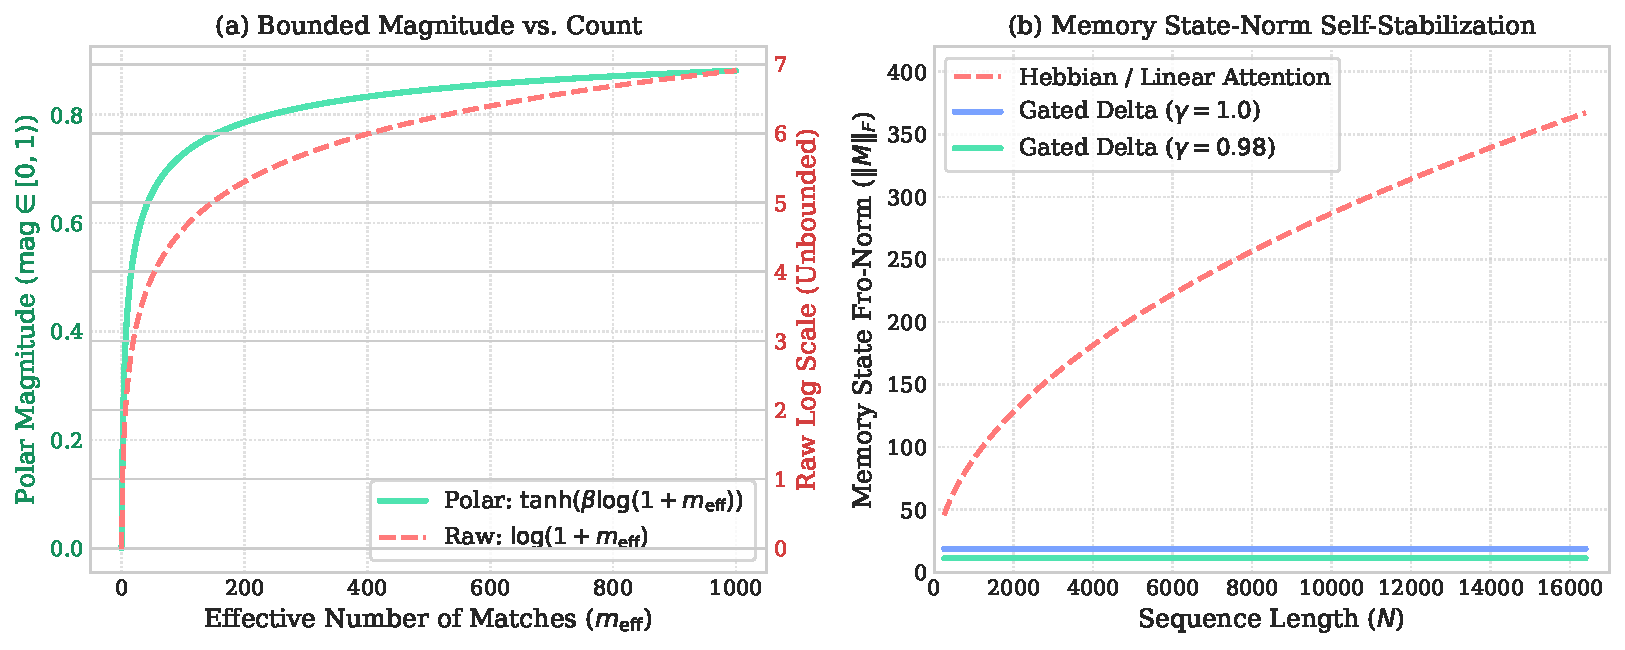
\includegraphics[width=\linewidth]{fig_machinery.pdf}
\caption{Mechanistic behavior of the ATMA sequence-mixer. (a) Under Polar Attention, the count channel maps the effective number of matches $m_{\text{eff}}$ monotonically to a bounded interval $[0, 1)$ using a saturating $\tanh$ function, preventing representation shift. (b) In the Titans memory branch, the gated-delta recurrence self-stabilizes, keeping the state norm $\|M\|_F$ flat across long context sequences, whereas a standard Hebbian/linear-attention memory exhibits square-root growth ($\approx \sqrt{N}$), leading to divergence.}
\label{fig:machinery}
\end{figure}

\section{Experimental Setup}
To evaluate the length-extrapolation and retrieval capabilities of ATMA, we perform a massive factorial sweep across 100 distinct configurations.

\subsection{Model Configuration and Training}
All ablation candidates share a fixed model architecture to isolate the impact of the sequence mixer:
\begin{itemize}
    \item \textbf{Parameters:} 369.72M non-embedding parameters.
    \item \textbf{Layers:} 16 layers (12 LFM2 gated convolutions, 4 Attention layers).
    \item \textbf{Dimensions:} Hidden size $d_{\text{model}} = 1024$, head dimension $d_k = d_v = 128$.
    \item \textbf{Heads:} 8 query heads, 2 KV heads (Grouped Query Attention ratio of 1:4).
    \item \textbf{Vocabulary:} 50,304 (GPT-2 tokenizer).
\end{itemize}

We train each candidate for exactly 1B tokens (1 epoch) on the Fineweb-Edu corpus, using a sequence length of 2048. We utilize the advanced Muon optimizer for coordinate-descent weight updates on the sequence-mixer and MLP blocks, combined with AdamW on embedding and normalization layers. The learning rate uses a cosine schedule with a 70\% cooldown fraction.

\subsection{Ablation Grid Axes}
Our 100-run factorial sweep evaluates combinations across five categorical axes:
\begin{enumerate}
    \item \textbf{Attention Type} (\texttt{attn\_type}): \texttt{polar} (our proposed Polar Attention), \texttt{rope} (standard softmax attention with Rotary Position Embeddings \citep{rope2021}), and \texttt{nope} (softmax attention without positional encodings, which organically develop positional representations in causal transformers \citep{haviv2022transformer, wang2024length, zuo-etal-2025-position}, relying on LFM2 convolutions for spatial awareness).
    \item \textbf{Regularizer Mode} (\texttt{reg\_mode}): \texttt{baseline}, \texttt{weak}, \texttt{strong}, \texttt{discrete}, and \texttt{zipfian} (varying the strength and layout of signature-stream regularization).
    \item \textbf{Distractor Loss} (\texttt{distractor}): \texttt{off} vs \texttt{on} (calibrating the null floor with $R = 2048$ random keys).
    \item \textbf{Memory Branch} (\texttt{memory}): \texttt{off} vs \texttt{on} (enabling the Gated-Delta Titans memory branch).
    \item \textbf{Sliding Window} (\texttt{window}): \texttt{off} (full global attention) vs \texttt{on} (sliding window of width 1024 on the attention core).
\end{enumerate}

\subsection{Evaluation Probes}
Each trained model is evaluated across sequence multipliers from 1$\times$ to 32$\times$ the training length (2,048 to 65,536 tokens) using two critical probes:
\begin{enumerate}
    \item \textbf{Document Perplexity:} Measured on single, coherent long documents from the FinePDFs corpus. 
    \item \textbf{Induction Needle-in-a-Haystack:} We plant an induction needle (e.g., a specific key-value pattern like ``when the wolf sings, the sky turns [COLOR]'') early in a long text haystack, and query the model for the target color at varying context distances up to 64K tokens.
\end{enumerate}

\section{Experimental Results and Analysis}

\subsection{The Attention Generalization Failure}
We first analyze the performance of attention-only models (with no memory branch or windowing). Table~\ref{table:attention_alone} highlights a stark collapse in both perplexity and retrieval as sequence length exceeds the training threshold.

\begin{table}[h]
\centering
\begin{tabular}{lcccc}
\toprule
\textbf{Length (Multiplier)} & \textbf{Softmax PPL} & \textbf{Polar PPL} & \textbf{Softmax Needle} & \textbf{Polar Needle} \\
\midrule
2,048 (1$\times$)  & 2.76 & 2.83 & 98\% & 96\% \\
8,192 (4$\times$)  & 2.67 & 3.32 & 28\% & 15\% \\
32,768 (16$\times$) & 3.38 & 3.60 & 3\%  & 3\%  \\
65,536 (32$\times$) & 3.71 & 3.60 & 1\%  & 0\%  \\
\bottomrule
\end{tabular}
\caption{Performance of memoryless, windowless attention models. Both softmax and polar attention alone degrade rapidly in perplexity and experience complete retrieval collapse past 4$\times$ training length.}
\label{table:attention_alone}
\end{table}

This baseline diagnosis reveals that attention alone cannot generalize. Softmax dilutes its attention probability as context grows, while the polar core's unconstrained participation ratio $n_{\text{eff}}$ shifts the activation range, pushing downstream layers out-of-distribution.

\subsection{The Titans Memory Unlock}
Enabling the recurrent Titans gated-delta memory branch on top of the global Polar Attention core completely reverses this trend. The results for our winning configuration (\textbf{full polar + Titans memory, no window, no distractor}) are shown in Table~\ref{table:memory_unlock}.

\begin{table}[h]
\centering
\begin{tabular}{lcccc}
\toprule
\textbf{Needle Distance} & \textbf{Polar (No Mem)} & \textbf{Softmax + Mem} & \textbf{Polar + Mem (Ours)} & \textbf{Polar + Mem PPL} \\
\midrule
2,048 (1$\times$)  & 96\% & 98\% & 91\% & 2.70 \\
4,096 (2$\times$)  & 40\% & 98\% & 95\% & 2.45 \\
8,192 (4$\times$)  & 15\% & 94\% & 93\% & 2.22 \\
16,384 (8$\times$) & 8\%  & 85\% & \textbf{98\%} & 2.09 \\
32,768 (16$\times$)& 3\%  & 48\% & \textbf{96\%} & 2.01 \\
65,536 (32$\times$)& 0\%  & 16\% & \textbf{93\%} & \textbf{1.96} \\
\bottomrule
\end{tabular}
\caption{Retrieval accuracy and perplexity comparison under long-context extrapolation. The Polar + Titans memory hybrid holds retrieval accuracy above 90\% out to 64K, while document perplexity improves monotonically.}
\label{table:memory_unlock}
\end{table}

The combination of Polar Attention and Titans memory achieves the best of both worlds:
\begin{enumerate}
    \item \textbf{Monotonic Perplexity Reduction:} Document perplexity falls consistently from 2.70 nats down to 1.96 nats at 64K tokens, demonstrating that the model actively uses the longer context to improve predictions.
    \item \textbf{Flat Retrieval Generalization:} Retrieval accuracy remains flat at 91--98\% (length-weighted average of 94\%) out to 32$\times$ training length.
    \item \textbf{Polar vs. Softmax Contrast:} While Softmax + Titans memory performs well at shorter context lengths, it collapses to 16\% retrieval at 64K. This collapse occurs because the softmax representation is not length-invariant, leading to activation drift that corrupts the memory readout.
\end{enumerate}

\subsection{Ablation of Windowing and Distractors}
Surprisingly, when the memory branch is active, adding sliding windowing or distractor losses actually \textit{hurts} retrieval, as shown in Table~\ref{table:window_ablation}.

\begin{table}[h]
\centering
\begin{tabular}{lccc}
\toprule
\textbf{Needle Distance} & \textbf{Polar + Mem (Winner)} & \textbf{+ Distractor} & \textbf{+ Window (1024)} \\
\midrule
2,048 (1$\times$)  & \textbf{91\%} & 74\% & 51\% \\
16,384 (8$\times$) & \textbf{98\%} & 76\% & 53\% \\
65,536 (32$\times$)& \textbf{93\%} & 59\% & 30\% \\
\bottomrule
\end{tabular}
\caption{Impact of sliding-window and distractor loss when the memory is enabled. Windowing makes the attention core blind past width 1024, and the distractor over-corrects the floor, both harming retrieval.}
\label{table:window_ablation}
\end{table}

A sliding window restricts the attention layer from training on long-context patterns, making it unable to align its projections for distant keys. The distractor loss over-sharpens the null floor, which suppresses the weak but necessary signals retrieved from the long-term memory. Thus, the simplest configuration (full polar + memory) is strictly superior.

\subsection{Hardware-Software Codesign and Kernel Machinery}
To ensure that ATMA's mathematical properties translate into real-world efficiency, we perform a hardware-software codesign. We optimize the sequence mixers by implementing custom GPU kernels using the Triton programming language, integrating them across our training, reference, and paged inference pipelines.

\subsubsection{Fused Triton Polar Attention Kernel}
Standard attention implementations fail to handle Polar Attention efficiently due to the $O(T^2)$ memory cost of materializing the participation ratio's intermediate scores. To achieve $O(\text{block})$ memory in both the forward and backward passes, we implement a fused FlashAttention-style Triton kernel with query- and key-blocking.

To compute the participation ratio online, we must track an extra streamed accumulator $Q^2 = \sum_j \exp(\mathrm{temp} \cdot \sigma_{ij} - M)^2$ alongside the standard running max $M$ and denominator sum $L = \sum_j \exp(\mathrm{temp} \cdot \sigma_{ij} - M)$. On each max update from $M_{\text{old}}$ to $M_{\text{new}}$, we define the correction factor $\alpha = \exp(M_{\text{old}} - M_{\text{new}})$. The accumulators are rescaled as follows:
\begin{align}
    L &\leftarrow \alpha \cdot L \\
    S &\leftarrow \alpha \cdot S \\
    Q^2 &\leftarrow \alpha^2 \cdot Q^2
\end{align}
The squared correction factor $\alpha^2$ corrects the quadratic term in the participation ratio denominator. This enables exact numerical recovery of the participation ratio $n_{\text{eff}} = L^2 / Q^2$ at the end of the streaming reduction. The backward pass splits work by running a cheap query preamble in PyTorch and executing the heavy $O(T^2)$ gradient loops ($dq$, $dk/dv$) as optimized Triton loops, running \textbf{7--27$\times$ faster} and using \textbf{5$\times$ less peak memory} than the PyTorch eager baseline on an NVIDIA L4 GPU.

\subsubsection{GQA-Grouped Paged Polar Decode Kernel}
During the decode phase of inference, standard sequence mixers suffer from significant high-bandwidth memory (HBM) bottlenecks due to gathering paged KV cache buffers. We implement a custom \texttt{polar\_attention\_decode} kernel that reads directly from paged KV cache blocks using a sequence block table, making it completely CUDA-graph-capturable.

To maximize throughput, the kernel is \textbf{GQA-grouped}: a single threadblock serves a sequence and an entire KV head group. The block table loads the cached keys and values once into shared memory, and uses them to compute the scores for all 4 associated query heads in parallel, reducing HBM read traffic by 4$\times$. Furthermore, the key loop is dynamically bounded by the live context length rather than a graph-padded maximum sequence length, minimizing unnecessary flops during early generation steps.

\subsubsection{In-Place Recurrent Gated-Delta Step Kernel}
The recurrent Titans memory state represents a size $H \times d_k \times d_v$ tensor per sequence-layer (approx. 512 KB/seq/layer at FP32), making memory updates the dominant decode bottleneck at large batch sizes. Standard implementations gather the recurrent state, perform a batched matrix-update kernel, and scatter the state back, incurring massive HBM traffic.

To address this, we implement a fused, in-place gated-delta step kernel (\texttt{kernel/gated\_delta\_triton.py}). During each decode step, the kernel loads the sequence state, computes the rank-1 gated-delta write $M_t = \gamma_t M_{t-1}(I - \beta_t k_t k_t^{\top}) + \beta_t v_t k_t^{\top}$ in-place, and writes the updated state directly back to the slot-indexed sequence state table. This eliminates the gather-scatter cycle entirely, reducing memory traffic by 3$\times$.

\subsubsection{Empirical Systems Performance and Overhead}
We evaluate our systems optimizations on an NVIDIA L4 GPU (24GB).
\begin{itemize}
    \item \textbf{Training Efficiency (MFU):} The gated-delta recurrence contains sequential cross-step dependencies that force PyTorch Dynamo compiler graph breaks. We wrap the Flash Linear Attention forward and backward passes as opaque custom ops (\texttt{FLA\_CUSTOM\_OP=1}) with fake shape registrations. This allows Dynamo to compile the surrounding layers cleanly and enables backward activation recomputation. As shown in Table~\ref{table:mfu_overhead}, the entire recurrent memory branch adds only \textbf{6--9\% relative MFU overhead} to training.
    \item \textbf{Inference Throughput:} Our GQA-grouped paged decode kernel and in-place gated-delta step kernel achieve a decode throughput of \textbf{19,270 tokens/second} at a batch size of 512.
\end{itemize}

\begin{table}[h]
\centering
\begin{tabular}{lccc}
\toprule
\textbf{Configuration} & \textbf{MFU without Memory} & \textbf{MFU with Memory} & \textbf{Relative Cost} \\
\midrule
+ Distractor ($R=2048$) & 30.1\% & 28.4\% & $\approx$ 6.0\% \\
No Distractor           & 36.1\% & 32.9\% & $\approx$ 8.9\% \\
\bottomrule
\end{tabular}
\caption{Model Flops Utilization (MFU) of ATMA training with and without the memory branch on NVIDIA L4 GPUs. Our systems optimizations keep the training overhead minimal.}
\label{table:mfu_overhead}
\end{table}

\section{Conclusion}
We presented ATMA, a hybrid sequence mixer that resolves the long-context perplexity-retrieval trade-off. By pairing a length-invariant Polar Attention core with a recurrent gated-delta Titans memory, ATMA retains flat induction needle retrieval accuracy above 90\% out to 64K tokens (32$\times$ training length) while document perplexity reduces monotonically. We rigorously verified our design through a 100-run sweep, and demonstrated that hardware-level software codesign restricts the memory's computational cost to under 9\% of the training budget. Future work will investigate extending write-path distractors to further enhance memory capacity.

\bibliography{colm2026_conference}
\bibliographystyle{colm2026_conference}

\appendix
\section{Complete Ablation Sweep Results}
We present the full numerical results of our 100-run factorial ablation sweep. The table lists the attention type, signature-stream regularization mode, distractor status, memory branch status, sliding-window status, training validation loss, document perplexity at multipliers 1$\times$ and 32$\times$ (2K and 64K tokens), needle-in-a-haystack retrieval accuracy at 2K and 64K tokens, and training Model Flops Utilization (MFU).

\begin{landscape}
\begin{longtable}{llcccrccccc}
\caption{Complete Results of the 100-Run Ablation Sweep. All models are 370M parameters, trained on FineWeb-Edu for 1B tokens ($seq\_len=2048$). Evaluated from 2K to 64K context length. PPL is in nats (lower is better), Needle is accuracy in \% (higher is better), MFU is training model flops utilization in \%. \label{table:ablation_appendix}}\\
\toprule
Type & Reg & Dist & Mem & Win & Val Loss & PPL@2K & PPL@64K & Needle@2K & Needle@64K & MFU \\
\midrule
\endfirsthead
\caption[]{Complete Results of the 100-Run Ablation Sweep (continued).}\\
\toprule
Type & Reg & Dist & Mem & Win & Val Loss & PPL@2K & PPL@64K & Needle@2K & Needle@64K & MFU \\
\midrule
\endhead
\midrule
\multicolumn{11}{r}{{Continued on next page}} \\
\bottomrule
\endfoot
\bottomrule
\endlastfoot
POLAR & baseline & Off & Off & Off & 3.323 & 2.83 & 3.60 & 96.3 & 0.0 & 40.1 \\
POLAR & baseline & Off & Off & On & 3.343 & 2.83 & 2.66 & 67.5 & 0.0 & 39.6 \\
POLAR & baseline & Off & On & Off & 3.169 & 2.70 & 1.96 & 91.3 & 92.5 & 35.6 \\
POLAR & baseline & Off & On & On & 3.174 & 2.71 & 2.01 & 51.3 & 30.0 & 35.6 \\
POLAR & baseline & On & Off & Off & 3.332 & 2.81 & 5.56 & 85.0 & 0.0 & 33.3 \\
POLAR & baseline & On & Off & On & 3.361 & 2.85 & 2.89 & 91.3 & 2.5 & 34.5 \\
POLAR & baseline & On & On & Off & 3.178 & 2.72 & 1.98 & 73.8 & 58.8 & 31.8 \\
POLAR & baseline & On & On & On & 3.182 & 2.73 & 1.97 & 56.3 & 21.3 & 31.2 \\
POLAR & weak & Off & Off & Off & 3.333 & 2.82 & 2.86 & 88.8 & 0.0 & 39.0 \\
POLAR & weak & Off & Off & On & 3.348 & 2.90 & 3.76 & 93.8 & 0.0 & 37.9 \\
POLAR & weak & Off & On & Off & 3.179 & 2.74 & 1.95 & 70.0 & 51.3 & 36.2 \\
POLAR & weak & Off & On & On & 3.187 & 2.74 & 1.99 & 41.3 & 41.3 & 36.2 \\
POLAR & weak & On & Off & Off & 3.335 & 2.82 & 3.47 & 91.3 & 0.0 & 32.8 \\
POLAR & weak & On & Off & On & 3.353 & 2.82 & 2.58 & 96.3 & 1.3 & 32.8 \\
POLAR & weak & On & On & Off & 3.178 & 2.74 & 1.95 & 33.8 & 32.5 & 30.7 \\
POLAR & weak & On & On & On & 3.183 & 2.74 & 1.94 & 81.3 & 78.8 & 30.7 \\
POLAR & strong & Off & Off & Off & 3.338 & 2.85 & 3.79 & 98.8 & 1.3 & 37.3 \\
POLAR & strong & Off & Off & On & 3.360 & 2.85 & 2.99 & 91.3 & 0.0 & 37.9 \\
POLAR & strong & Off & On & Off & 3.172 & 2.72 & 1.96 & 80.0 & 52.5 & 35.8 \\
POLAR & strong & Off & On & On & 3.181 & 2.72 & 1.94 & 76.3 & 68.8 & 34.6 \\
POLAR & strong & On & Off & Off & 3.337 & 2.87 & 3.22 & 83.8 & 1.3 & 32.8 \\
POLAR & strong & On & Off & On & 3.347 & 2.82 & 2.64 & 97.5 & 16.3 & 32.2 \\
POLAR & strong & On & On & Off & 3.179 & 2.73 & 1.94 & 86.3 & 83.8 & 30.9 \\
POLAR & strong & On & On & On & 3.182 & 2.72 & 1.94 & 25.0 & 23.8 & 30.9 \\
POLAR & discrete & Off & Off & Off & 3.338 & 2.82 & 2.80 & 93.8 & 2.5 & 37.9 \\
POLAR & discrete & Off & Off & On & 3.349 & 2.87 & 2.90 & 93.8 & 6.3 & 37.9 \\
POLAR & discrete & Off & On & Off & 3.184 & 2.75 & 2.03 & 76.3 & 73.8 & 36.4 \\
POLAR & discrete & Off & On & On & 3.178 & 2.71 & 1.92 & 31.3 & 18.8 & 35.8 \\
POLAR & discrete & On & Off & Off & 3.333 & 2.80 & 4.13 & 97.5 & 0.0 & 32.6 \\
POLAR & discrete & On & Off & On & 3.351 & 2.87 & 2.72 & 85.0 & 2.5 & 33.3 \\
POLAR & discrete & On & On & Off & 3.189 & 2.74 & 1.96 & 87.5 & 53.8 & 31.8 \\
POLAR & discrete & On & On & On & 3.192 & 2.74 & 2.07 & 21.3 & 26.3 & 31.7 \\
POLAR & zipfian & Off & Off & Off & 3.338 & 2.85 & 4.83 & 96.3 & 11.3 & 37.9 \\
POLAR & zipfian & Off & Off & On & 3.350 & 2.83 & 2.58 & 88.8 & 3.8 & 39.4 \\
POLAR & zipfian & Off & On & Off & 3.171 & 2.70 & 1.92 & 52.5 & 63.8 & 36.2 \\
POLAR & zipfian & Off & On & On & 3.180 & 2.75 & 1.95 & 46.3 & 40.0 & 35.2 \\
POLAR & zipfian & On & Off & Off & 3.340 & 2.83 & 3.77 & 98.8 & 1.3 & 33.8 \\
POLAR & zipfian & On & Off & On & 3.352 & 2.85 & 3.13 & 90.0 & 0.0 & 33.5 \\
POLAR & zipfian & On & On & Off & 3.177 & 2.72 & 1.94 & 91.3 & 67.5 & 31.8 \\
POLAR & zipfian & On & On & On & 3.192 & 2.74 & 2.00 & 40.0 & 26.3 & 31.8 \\
NOPE & baseline & Off & Off & Off & 3.224 & 2.76 & 3.71 & 97.5 & 1.3 & 41.5 \\
NOPE & baseline & Off & Off & On & 3.219 & 2.75 & 2.76 & 92.5 & 10.0 & 36.5 \\
NOPE & baseline & Off & On & Off & 3.140 & 2.66 & 2.34 & 97.5 & 16.3 & 36.8 \\
NOPE & baseline & Off & On & On & 3.150 & 2.70 & 2.14 & 81.3 & 0.0 & 34.2 \\
NOPE & baseline & On & Off & Off & 3.209 & 2.74 & 2.99 & 90.0 & 18.8 & 32.5 \\
NOPE & baseline & On & Off & On & 3.212 & 2.77 & 2.90 & 81.3 & 0.0 & 30.3 \\
NOPE & baseline & On & On & Off & 3.149 & 2.67 & 2.35 & 80.0 & 16.3 & 30.0 \\
NOPE & baseline & On & On & On & 3.147 & 2.68 & 2.09 & 88.8 & 21.3 & 28.2 \\
NOPE & weak & Off & Off & Off & 3.214 & 2.77 & 3.10 & 95.0 & 0.0 & 40.9 \\
NOPE & weak & Off & Off & On & 3.222 & 2.75 & 3.05 & 81.3 & 0.0 & 36.1 \\
NOPE & weak & Off & On & Off & 3.147 & 2.68 & 2.07 & 88.8 & 21.3 & 37.5 \\
NOPE & weak & Off & On & On & 3.142 & 2.68 & 2.12 & 82.5 & 0.0 & 33.7 \\
NOPE & weak & On & Off & Off & 3.215 & 2.75 & 4.87 & 95.0 & 5.0 & 32.0 \\
NOPE & weak & On & Off & On & 3.221 & 2.73 & 2.63 & 81.3 & 0.0 & 29.3 \\
NOPE & weak & On & On & Off & 3.147 & 2.67 & 2.48 & 97.5 & 1.3 & 30.8 \\
NOPE & weak & On & On & On & 3.148 & 2.68 & 2.14 & 93.8 & 1.3 & 28.4 \\
NOPE & strong & Off & Off & Off & 3.231 & 2.74 & 4.88 & 90.0 & 2.5 & 38.4 \\
NOPE & strong & Off & Off & On & 3.214 & 2.72 & 2.68 & 82.5 & 0.0 & 36.4 \\
NOPE & strong & Off & On & Off & 3.144 & 2.68 & 2.37 & 96.3 & 6.3 & 35.7 \\
NOPE & strong & Off & On & On & 3.150 & 2.70 & 2.10 & 93.8 & 7.5 & 33.8 \\
NOPE & strong & On & Off & Off & 3.207 & 2.72 & 3.13 & 73.8 & 0.0 & 31.4 \\
NOPE & strong & On & Off & On & 3.214 & 2.74 & 2.49 & 86.3 & 8.8 & 28.9 \\
NOPE & strong & On & On & Off & 3.146 & 2.67 & 2.24 & 83.8 & 17.5 & 29.1 \\
NOPE & strong & On & On & On & 3.147 & 2.68 & 2.16 & 96.3 & 0.0 & 27.5 \\
NOPE & discrete & Off & Off & Off & 3.202 & 2.75 & 3.33 & 85.0 & 1.3 & 38.8 \\
NOPE & discrete & Off & Off & On & 3.234 & 2.79 & 3.11 & 70.0 & 18.8 & 37.0 \\
NOPE & discrete & Off & On & Off & 3.145 & 2.68 & 2.14 & 98.8 & 16.3 & 36.0 \\
NOPE & discrete & Off & On & On & 3.145 & 2.68 & 2.10 & 95.0 & 3.8 & 34.3 \\
NOPE & discrete & On & Off & Off & 3.212 & 2.88 & 3.04 & 42.5 & 0.0 & 31.2 \\
NOPE & discrete & On & Off & On & 3.211 & 2.78 & 2.73 & 82.5 & 1.3 & 29.1 \\
NOPE & discrete & On & On & Off & 3.145 & 2.68 & 2.27 & 91.3 & 11.3 & 30.3 \\
NOPE & discrete & On & On & On & 3.149 & 2.68 & 2.17 & 83.8 & 0.0 & 28.6 \\
NOPE & zipfian & Off & Off & Off & 3.209 & 2.71 & 3.18 & 90.0 & 0.0 & 40.8 \\
NOPE & zipfian & Off & Off & On & 3.219 & 2.75 & 2.71 & 77.5 & 1.3 & 36.1 \\
NOPE & zipfian & Off & On & Off & 3.141 & 2.67 & 2.55 & 96.3 & 0.0 & 38.0 \\
NOPE & zipfian & Off & On & On & 3.150 & 2.69 & 2.11 & 90.0 & 3.8 & 33.7 \\
NOPE & zipfian & On & Off & Off & 3.207 & 2.77 & 3.32 & 82.5 & 0.0 & 31.3 \\
NOPE & zipfian & On & Off & On & 3.227 & 2.79 & 2.91 & 93.8 & 11.3 & 30.2 \\
NOPE & zipfian & On & On & Off & 3.146 & 2.68 & 2.39 & 96.3 & 21.3 & 29.6 \\
NOPE & zipfian & On & On & On & 3.148 & 2.68 & 2.17 & 90.0 & 6.3 & 28.7 \\
ROPE & baseline & Off & Off & Off & 3.159 & 2.85 & 3.36 & 42.5 & 0.0 & 40.4 \\
ROPE & baseline & Off & Off & On & 3.163 & 2.86 & 3.79 & 15.0 & 0.0 & 37.2 \\
ROPE & baseline & Off & On & Off & 3.145 & 2.81 & 2.86 & 73.8 & 0.0 & 37.1 \\
ROPE & baseline & Off & On & On & 3.151 & 2.80 & 2.95 & 13.8 & 0.0 & 34.4 \\
ROPE & baseline & On & Off & Off & 3.163 & 3.00 & 3.47 & 38.8 & 0.0 & 33.2 \\
ROPE & baseline & On & Off & On & 3.167 & 2.88 & 4.06 & 0.0 & 0.0 & 30.2 \\
ROPE & baseline & On & On & Off & 3.153 & 2.73 & 2.45 & 75.0 & 0.0 & 31.4 \\
ROPE & baseline & On & On & On & 3.154 & 2.83 & 2.86 & 32.5 & 0.0 & 29.4 \\
ROPE & strong & Off & Off & Off & 3.165 & 2.78 & 3.34 & 30.0 & 0.0 & 39.0 \\
ROPE & strong & Off & On & Off & 3.158 & 2.85 & 2.63 & 51.3 & 0.0 & 35.9 \\
ROPE & strong & Off & On & On & 3.162 & 2.86 & 3.08 & 10.0 & 0.0 & 33.2 \\
ROPE & strong & On & Off & Off & 3.161 & 2.85 & 3.58 & 47.5 & 0.0 & 31.1 \\
ROPE & strong & On & On & On & 3.162 & 2.85 & 3.08 & 2.5 & 0.0 & 28.4 \\
ROPE & discrete & Off & Off & Off & 3.165 & 2.91 & 3.43 & 22.5 & 0.0 & 39.7 \\
ROPE & discrete & Off & Off & On & 3.158 & 2.84 & 4.05 & 3.8 & 0.0 & 36.9 \\
ROPE & discrete & Off & On & Off & 3.159 & 2.83 & 2.67 & 47.5 & 0.0 & 36.3 \\
ROPE & discrete & Off & On & On & 3.161 & 2.79 & 2.71 & 41.3 & 0.0 & 33.7 \\
ROPE & discrete & On & Off & On & 3.164 & 2.80 & 3.74 & 21.3 & 0.0 & 30.0 \\
ROPE & discrete & On & On & Off & 3.162 & 2.74 & 2.47 & 50.0 & 0.0 & 30.9 \\
ROPE & discrete & On & On & On & 3.154 & 2.79 & 2.68 & 18.8 & 0.0 & 28.9 \\
\end{longtable}

\end{landscape}

\end{document}
